\documentclass[journal]{IEEEtran}

\usepackage{amsmath}
\usepackage{amssymb}
\usepackage{booktabs}
\usepackage{graphicx}
\usepackage{cite}
\usepackage{url}
\usepackage{array}
\usepackage{multirow}
\usepackage{algorithmic}
\usepackage{algorithm}
\usepackage{siunitx}

\graphicspath{{figures/}}

\begin{document}

\title{Scaling Hierarchical Coordination for Million-Unit Space Swarms: Discrete Event Simulation and Architectural Analysis}

\author{
  \IEEEauthorblockN{Project Dyson Research Team}
  \IEEEauthorblockA{Project Dyson\\
  \url{https://projectdyson.org}}
}

\markboth{IEEE Transactions on Aerospace and Electronic Systems}{}

\maketitle

\begin{abstract}
Future space infrastructure concepts require coordination of $10^5$ to $10^6$ autonomous nodes---scales at which no coordination architecture has been systematically evaluated. We present a discrete event simulation (DES) comparing centralized, hierarchical, and mesh topologies at scales from $10^3$ to $10^6$ spacecraft. Centralized architectures face two bottlenecks: processing latency (addressable via parallelization, with the single-server limit at ${\sim}10{,}000$ nodes scaling linearly with server count) and fundamental physical constraints including propagation delay and spectrum scarcity. Mesh topologies parameterized for global state convergence incur $O(N^2)$ overhead exceeding 25\% of coordination bandwidth beyond $10^5$ nodes. Hierarchical coordination, employing clusters of 50--100 nodes with rotating coordinators, provides the most favorable scaling properties under these requirements, maintaining 2--8\% overhead past $10^6$ nodes. The optimal coordinator duty cycle is 24--48 hours; a parameter-dependent overhead inflection near 50{,}000 nodes marks the onset of necessary optimizations. An AI-assisted exploration generated the Shepherd/Flock heterogeneous hardware concept. We discuss applicability to mega-constellations, drone swarms, and sensor networks.
\end{abstract}

\begin{IEEEkeywords}
Space systems coordination, swarm robotics, hierarchical control, discrete event simulation, mega-constellations, autonomous spacecraft, multi-agent systems
\end{IEEEkeywords}

%% ===========================================================================
%% SECTION 1: INTRODUCTION
%% ===========================================================================
\section{Introduction}

\subsection{The Coordination Scaling Problem}

The coordination of large numbers of autonomous spacecraft represents one of the significant open challenges in aerospace systems engineering. The largest operational constellation today, SpaceX's Starlink network, manages approximately 7{,}000 active satellites (as of mid-2024) through centralized ground-based coordination \cite{starlink_ops}. While this approach has proven effective at current scale, the system already requires substantial ground infrastructure and has encountered coordination challenges during conjunction events \cite{esa_conjunction}. Approved expansion plans for Starlink alone envision 42{,}000 satellites, and other operators including Amazon's Project Kuiper and OneWeb are deploying their own constellations \cite{kuiper, oneweb_mgmt}.

Looking further ahead, proposed space infrastructure concepts---including space-based solar power arrays and orbital manufacturing facilities---contemplate fleets of $10^5$ to $10^6$ autonomous units in the near term, with aspirational concepts such as Dyson swarm precursors potentially requiring far larger fleets in the long term \cite{oneil_1976, badescu_2006}. At these scales, the coordination problem is not merely a larger version of current constellation management; it is qualitatively different. Message processing latency, bandwidth allocation, state synchronization, and failure recovery all exhibit nonlinear scaling behaviors that can render architectures adequate at $10^3$ nodes entirely unworkable at $10^6$ \cite{lynch_distributed}.

No prior work has systematically compared coordination architectures across this range of scales using quantitative simulation. The literature on swarm robotics has extensively studied coordination at scales of tens to hundreds of agents \cite{brambilla_2013}, and constellation management literature addresses systems of up to approximately 10{,}000 nodes \cite{wertz_smad}, but the intermediate regime of $10^4$ to $10^6$ nodes remains largely unexplored.

\subsection{Research Questions}

This study addresses three interrelated research questions:

\begin{enumerate}
    \item[\textbf{RQ1:}] How do centralized, hierarchical, and mesh coordination architectures scale in terms of communication overhead, message latency, and failure resilience as fleet size increases from $10^3$ to $10^6$ nodes?
    \item[\textbf{RQ2:}] What is the optimal duty cycle for rotating cluster coordinators in a hierarchical architecture, considering the trade-off between handoff overhead and single-point-of-failure exposure?
    \item[\textbf{RQ3:}] At what fleet size do coordination constraints begin to dominate operational overhead, and what optimizations are necessary beyond this threshold?
\end{enumerate}

\subsection{Contributions}

The principal contributions of this paper are:
\begin{itemize}
    \item The first comparative discrete event simulation of coordination topologies at scales spanning three orders of magnitude ($10^3$ to $10^6$);
    \item Quantified communication overhead, message processing latency, and failure resilience characteristics for each topology as a function of scale;
    \item Identification of an optimal 24--48 hour coordinator duty cycle with associated power and reliability trade-off characterization;
    \item Establishment of a 50{,}000-node inflection point beyond which advanced optimizations become necessary;
    \item AI-assisted architectural exploration through a multi-model deliberation process, yielding the Shepherd/Flock heterogeneous hardware concept; and
    \item Practical design guidelines applicable to near-term mega-constellation management.
\end{itemize}


%% ===========================================================================
%% SECTION 2: RELATED WORK
%% ===========================================================================
\section{Related Work}

\subsection{Constellation Coordination}

Current satellite constellation management relies predominantly on centralized ground-based coordination. SpaceX operates Starlink through a network of ground stations and a centralized mission control that computes orbit adjustments, manages conjunction avoidance, and coordinates spectrum sharing \cite{starlink_ops}. The European Space Agency's Space Debris Office coordinates conjunction warnings across multiple operators, but the computational burden scales linearly with constellation size \cite{esa_conjunction}. OneWeb employs a similar centralized paradigm for its constellation management \cite{oneweb_mgmt}. All of these systems operate at fewer than 15{,}000 nodes, and none has published evidence of architectural scalability beyond this regime.

The Iridium constellation, while smaller at 66 active satellites, introduced inter-satellite links (ISLs) that reduced dependence on ground control for routine operations \cite{iridium_arch}. Handley~\cite{handley_2018} analyzed ISL routing topologies for mega-constellations such as Starlink, demonstrating that laser ISLs can provide lower latency than terrestrial fiber for long-distance paths, but did not address the coordination scaling problem. This partial decentralization foreshadowed the architectural direction explored in the present study, although Iridium's crosslink topology is fixed and would not scale to large swarm configurations.

\subsection{Swarm Robotics}

The swarm robotics literature provides a rich foundation for decentralized coordination. Brambilla et al.~\cite{brambilla_2013} present a comprehensive taxonomy of swarm behaviors, noting that most experimental demonstrations involve 10--100 agents with a few reaching 1{,}000. Dorigo et al.~\cite{dorigo_2021} survey the state of the art in swarm engineering, emphasizing the gap between theoretical scalability claims and experimental validation. Reynolds' seminal work on flocking behaviors \cite{reynolds_1987} demonstrated that simple local rules can produce emergent global coordination, but the computational analysis assumed homogeneous agents with identical sensing capabilities---an assumption that breaks down when heterogeneous coordination roles are required.

Bio-inspired approaches including ant colony optimization \cite{dorigo_aco}, particle swarm optimization \cite{kennedy_pso}, and artificial bee colony algorithms \cite{karaboga_abc} have been applied to multi-agent coordination. However, these approaches are primarily optimization heuristics rather than operational coordination architectures, and their convergence properties at $10^6$-node scale have not been established.

\subsection{Mathematical Foundations}

Several theoretical frameworks underpin the analysis of large-scale coordination. Lamport's foundational work on logical clocks and event ordering in distributed systems \cite{lamport_clocks} establishes the theoretical basis for consistent coordination in networks without global time references---directly relevant to space swarms where light-speed delays preclude tight synchronization. Consensus protocols such as Raft \cite{ongaro_raft} provide mechanisms for coordinator election and state replication in the presence of failures, and inform the coordinator rotation scheme explored in our hierarchical model. Tolstaya et al.~\cite{tolstaya_gnn} demonstrated that Graph Neural Network (GNN) controllers for multi-robot systems achieve communication complexity that scales linearly with the number of agents, contrasting with the quadratic scaling of naive broadcast approaches. This result provides a theoretical lower bound on the communication overhead achievable by any distributed coordination scheme.

Mean-field game theory, introduced by Lasry and Lions \cite{lasry_mfg} and independently by Huang et al.~\cite{huang_mfg}, offers a framework for analyzing systems with very large numbers of interacting agents by replacing individual agent tracking with statistical population descriptions. This approach is particularly relevant at the scales considered in this study, where tracking the state of every individual node becomes computationally intractable.

It is well established that hierarchical topologies achieve $O(\log N)$ information propagation time (an elementary consequence of tree depth) compared to $O(N)$ for flat mesh networks and $O(1)$ for centralized architectures (at the cost of a central bottleneck) \cite{lynch_distributed}. Li et al.~\cite{li_decentralized} demonstrate that GNN-based controllers can approach these theoretical bounds in practice for decentralized multi-robot path planning with limited communication. These results motivate the hierarchical topology explored in our simulation study.

\subsection{Military Drone Swarm Programs}

The DARPA Offensive Swarm-Enabled Tactics (OFFSET) program has demonstrated coordination of over 100 autonomous drones in field exercises \cite{darpa_offset}. The DARPA Blackjack program is developing autonomous satellite mesh networking for proliferated low-Earth-orbit constellations, explicitly targeting decentralized coordination without persistent ground connectivity \cite{darpa_blackjack}. The Naval Research Laboratory has conducted experiments with up to 250 coordinated UAVs \cite{nrl_swarm}. The Department of Defense Replicator initiative aims to field thousands of autonomous systems \cite{dod_replicator}. While these programs represent the state of the art in operational swarm coordination, none has published results at scales exceeding approximately 250 units for aerial systems, and the coordination architectures employed are typically centralized or use fixed hierarchical command structures. The SWIM protocol \cite{das_swim} provides an efficient failure detection mechanism for large distributed systems that could complement the coordinator-based failure detection in our hierarchical model.


%% ===========================================================================
%% SECTION 3: SIMULATION FRAMEWORK
%% ===========================================================================
\section{Simulation Framework}

\subsection{Discrete Event Simulation Architecture}

We implement a discrete event simulation (DES) framework in which autonomous nodes exchange messages according to the rules of one of three coordination topologies. The simulation is event-driven: no computation occurs between events, allowing efficient modeling of long operational periods. Each simulation run models one year of swarm operations.

The event types modeled are:
\begin{itemize}
    \item \textbf{Status reports}: periodic health and position telemetry from nodes to their coordinator (or broadcast, depending on topology);
    \item \textbf{Coordination messages}: task assignments, orbit adjustments, and cluster-level directives;
    \item \textbf{Handoff events}: transfer of coordinator responsibility between nodes (hierarchical topology only);
    \item \textbf{Failure events}: node failures, drawn from an exponential distribution;
    \item \textbf{Collision avoidance}: proximity alerts requiring time-critical response.
\end{itemize}

Events at both resolutions are managed through a single priority queue ordered by simulated time; one-second resolution applies only to collision avoidance events, while all other events (status reports, coordination messages, handoffs, failures) use one-minute resolution. Messages experience propagation delay proportional to inter-node distance (at light speed) plus processing delay at the receiving node, modeled as a service time drawn from the appropriate queueing model for each topology. We note that the communication model abstracts away MAC-layer scheduling, link acquisition, and pointing constraints that are significant in real space links \cite{ccsds_prox1}; these simplifications are discussed in Section~V-E.

\subsection{Topology Models}

\subsubsection{Centralized Topology}

In the centralized model, a single ground-based coordinator receives all status reports, computes coordination decisions, and issues commands to individual nodes. We model the coordinator as an $M/D/1$ queue with finite buffer \cite{kleinrock_queueing}:

\begin{equation}
    \rho = \frac{\lambda}{\mu} = \frac{N \cdot r}{C}
    \label{eq:centralized_utilization}
\end{equation}

\noindent where $N$ is the number of nodes, $r$ is the per-node reporting rate, $C$ is the coordinator's processing capacity (messages per second), and $\rho$ is the server utilization. The mean waiting time in the $M/D/1$ queue is:

\begin{equation}
    W_q = \frac{\rho}{2\mu(1 - \rho)}
    \label{eq:md1_waiting}
\end{equation}

As $\rho \to 1$, waiting time diverges. Our simulation parameterizes $C = 1{,}000$ messages per second for a single processing server, representative of a single ground station processing thread. At a reporting rate of $r = 0.1$ messages per second per node, utilization reaches $\rho = 1.0$ at $N = 10{,}000$.

This single-server model represents a \emph{worst-case bound} on centralized processing capacity. Real ground systems employ parallel processing across multiple servers, which can be modeled as an $M/D/c$ queue where $c$ is the number of parallel servers. In this case, utilization becomes:

\begin{equation}
    \rho_c = \frac{N \cdot r}{c \cdot C}
    \label{eq:mdc_utilization}
\end{equation}

\noindent and the scalability limit shifts to $N_{\max} = c \cdot C / r$. Table~\ref{tab:mdc_sensitivity} shows the resulting scalability limits for representative values of~$c$.

\begin{table}[t]
    \centering
    \caption{Centralized $M/D/c$ Scalability Sensitivity ($C = 1{,}000$~msg/s, $r = 0.1$~msg/s)}
    \label{tab:mdc_sensitivity}
    \begin{tabular}{@{}lcl@{}}
        \toprule
        \textbf{Servers $c$} & $\boldsymbol{N_{\max}}$ & \textbf{Representative System} \\
        \midrule
        1    & 10{,}000      & Single ground station thread \\
        10   & 100{,}000     & Multi-threaded ground station \\
        100  & 1{,}000{,}000 & Dedicated ground station cluster \\
        1000 & 10{,}000{,}000 & Hyperscale data center \\
        \bottomrule
    \end{tabular}
\end{table}

Processing capacity is thus addressable through parallelization: with sufficient ground infrastructure investment, the processing bottleneck alone does not preclude centralized coordination at any simulated scale. However, centralized architectures face a second, \emph{fundamental} class of bottleneck that parallelization cannot resolve:

\textbf{Propagation latency.} All coordination messages must traverse the ground-to-space link. At geostationary relay altitudes, this introduces a minimum 240~ms round-trip delay; even via low-Earth-orbit relay, 10--40~ms delays are unavoidable. For time-critical collision avoidance at closing velocities of km/s, these delays may exceed the decision window.

\textbf{Spectrum scarcity.} At $10^6$ nodes reporting at $r = 0.1$~msg/s with 256-byte status reports, the aggregate uplink data rate is $N \cdot r \cdot 256 \cdot 8 = 204.8$~Mbps for status telemetry alone. Adding downlink commands approximately doubles this to ${\sim}410$~Mbps total. A single Ka-band ground station typically provides 1--2~Gbps of aggregate throughput shared across all users; supporting $10^6$ nodes would therefore require a dedicated network of ground stations with substantial spectrum allocation---a resource that is finite and increasingly contested \cite{handley_2018}. Distributing coordination via inter-satellite links avoids this spectrum bottleneck entirely.

Our simulation uses the single-server parameterization ($c = 1$) to establish a conservative processing baseline. The results in Section~IV should be interpreted with the understanding that centralized processing limits scale linearly with~$c$, but that propagation latency and spectrum constraints impose architecture-level limits that are independent of ground infrastructure investment.

The total message complexity per coordination cycle is $O(N)$, as each node sends one report and receives one command.

\subsubsection{Hierarchical Topology}

The hierarchical model implements a four-level tree structure (Fig.~\ref{fig:architecture}):

\begin{figure}[t]
    \centering
    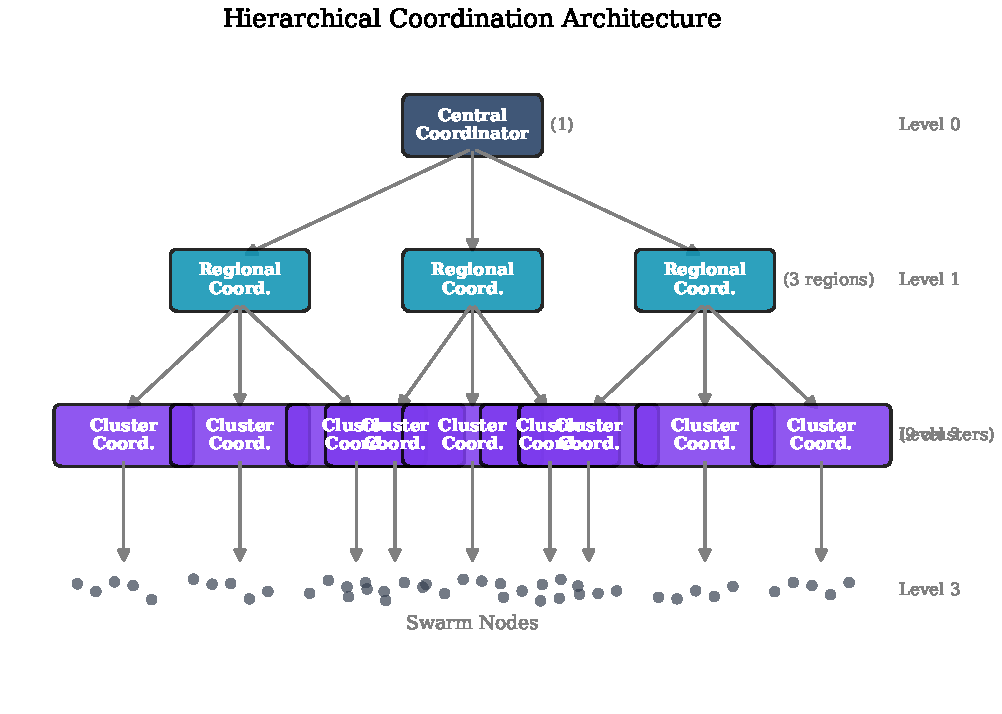
\includegraphics[width=\columnwidth]{fig-architecture-diagram.pdf}
    \caption{Four-level hierarchical coordination architecture. Ground control connects to 10--100 regional coordinators, each managing 10--100 cluster coordinators, each responsible for 50--100 individual nodes. Labels indicate message aggregation ratios at each level of the hierarchy.}
    \label{fig:architecture}
\end{figure}

\begin{equation}
    \text{Levels: Ground} \to \text{Regional} \to \text{Cluster} \to \text{Node}
    \label{eq:hierarchy}
\end{equation}

\noindent with configurable fan-out at each level. Nodes report to their cluster coordinator, which aggregates reports and forwards summaries to the regional coordinator, which in turn aggregates for the ground station. The aggregation ratio $\alpha$ at each level reduces message volume:

\begin{equation}
    M_{\text{total}} = N + \frac{N}{k_c} + \frac{N}{k_c \cdot k_r}
    \label{eq:hierarchical_messages}
\end{equation}

\noindent where $k_c$ is the cluster size and $k_r$ is the number of clusters per regional coordinator. For $k_c = 100$ and $k_r = 100$, the ground station processes only $N/10{,}000$ messages per cycle rather than $N$. Note that Eq.~\ref{eq:hierarchical_messages} counts upward reporting only; downward commands (task assignments, orbit adjustments relayed from regional to cluster to node) approximately double the total message count but do not change the asymptotic complexity.

With the fixed four-level hierarchy described above, the total message complexity per coordination cycle is $O(N)$: each level contributes $O(N)$ messages, and the number of levels is constant. This linear scaling is a key strength of the fixed-depth design, ensuring that coordination cost grows proportionally with fleet size without the logarithmic overhead that would arise if hierarchy depth were adapted dynamically. An adaptive hierarchy whose depth grew as $O(\log N)$ with fleet size would yield $O(N \log N)$ total complexity; we do not employ such a design, as the fixed four levels provide sufficient aggregation across the simulated range of $10^3$ to $10^6$ nodes.

To make the queueing model symmetric with the centralized $M/D/1$ specification (Eq.~\ref{eq:centralized_utilization}), we assign explicit service rates at each hierarchical level. The cluster coordinator processes $k_c$ node reports per cycle at $C_{\text{cluster}} = 200$~msg/s (reflecting limited on-board processing compared to ground infrastructure). The regional coordinator processes $N/k_c$ aggregated cluster reports at $C_{\text{regional}} = 500$~msg/s. The ground station processes $N/(k_c \cdot k_r)$ regional summaries at $C_{\text{ground}} = 1{,}000$~msg/s. The cluster coordinator is the first level to saturate, reaching $\rho = 1$ when $k_c \cdot r / C_{\text{cluster}} = 1$, i.e., at $k_c = C_{\text{cluster}} / r = 2{,}000$ nodes per cluster. Since our parameterization uses $k_c \leq 500$, the cluster coordinator operates well below saturation ($\rho \leq 0.25$). This headroom is what produces the U-shaped cluster size curve in Section~IV-B: overhead rises at small $k_c$ due to excessive inter-cluster traffic and at large $k_c$ because the cluster coordinator approaches its processing capacity.

Coordinator rotation is modeled as a state transfer event. The outgoing coordinator transmits its accumulated state (10--50~MB, depending on cluster size) to the incoming coordinator over an optical inter-satellite link at 1--10~Gbps, completing the handoff in 1--10~seconds. During the handoff window, the cluster operates in a degraded mode where routine coordination is deferred but collision avoidance remains active through direct node-to-node communication.

\subsubsection{Mesh Topology}

The mesh model implements a gossip protocol in which each node periodically selects a random subset of $f$ neighbors (the \emph{fanout}) and exchanges state information. In standard epidemic dissemination with constant fanout $f = O(1)$ or logarithmic fanout $f = O(\log N)$, convergence to full state dissemination requires $O(\log N)$ rounds, yielding total message complexities of $O(N \log N)$ or $O(N \log^2 N)$ respectively \cite{demers_gossip}.

However, the coordination scenario considered here requires \emph{global state convergence}: each node must maintain awareness of trajectories beyond its immediate orbital neighborhood to support fleet-wide coordination. Three astrodynamics considerations drive this requirement. First, coordinated orbit-raising maneuvers---essential during swarm deployment and station-keeping campaigns---affect the entire fleet simultaneously, as thrust applied by one group of nodes alters the conjunction geometry for all others. Second, intersecting orbital planes create non-local conjunction risks: a node in one plane may threaten a node in a different plane that is not a spatial neighbor at the time of planning but will be at the time of closest approach, hours or days later. Third, dense orbital shells with $10^5$+ objects exhibit conjunction cascades where an avoidance maneuver by one node creates secondary conjunction risks for distant nodes, requiring fleet-wide awareness to resolve safely.

In a swarm of $N$ nodes distributed across an orbital shell, each node must therefore eventually receive trajectory updates from all $O(N)$ nodes---not merely propagate a single rumor. When the state to be disseminated is the full $N$-node trajectory table, the total information that must flow through the network is $O(N^2)$ regardless of the gossip protocol used, because each of $N$ nodes must receive $O(N)$ state entries. With fanout $f = O(N / \log N)$, convergence occurs in $O(\log N)$ rounds:

\begin{equation}
    M_{\text{mesh}} = O(N \cdot f \cdot \log N) = O(N^2)
    \label{eq:mesh_messages}
\end{equation}

A locality-aware mesh using sectorized dissemination---where each node gossips primarily with orbital neighbors and relies on multi-hop forwarding for non-local updates---would reduce per-node overhead to $O(k)$ per round but would sacrifice coordination capability for fleet-wide operations. Convergence time for non-local state would grow to $O(D)$ gossip rounds (where $D$ is the network diameter), introducing staleness in the trajectory data used for cross-plane conjunction assessment. The $O(N^2)$ characterization thus represents the cost of the \emph{full global coordination requirement}; partial coordination via local mesh is addressed in our hierarchical model through intra-cluster gossip, where each cluster coordinator aggregates and disseminates non-local state to its members at a cost of $O(k_c)$ per node.

This distinction is important: the hierarchical topology avoids the $O(N^2)$ information-theoretic cost through aggregation, reducing the per-node information requirement from $O(N)$ to $O(k_c)$ (the cluster size) while preserving fleet-wide coordination capability through the coordinator hierarchy.

Convergence time scales with the network diameter $D$:

\begin{equation}
    T_{\text{converge}} = D \cdot \tau_{\text{gossip}}
    \label{eq:mesh_convergence}
\end{equation}

\noindent where $\tau_{\text{gossip}}$ is the gossip round interval. For a random geometric graph with $N$ nodes in three-dimensional orbital space, $D = O(N^{1/3})$.

\subsection{Node Model}

Each simulated node is characterized by the following parameters:

\begin{itemize}
    \item \textbf{Communication power}: 5~W baseline, 15--20~W in coordinator mode;
    \item \textbf{Bandwidth allocation}: 1~kbps per node for coordination traffic;
    \item \textbf{Failure model}: exponential inter-arrival times with a 2\% annual failure rate, yielding a mean time to failure (MTTF) of 50~years per node;
    \item \textbf{State vector}: position (3 components), velocity (3 components), health status, power level, and cluster assignment.
\end{itemize}

The failure rate of 2\% annually is consistent with observed rates for modern small satellites in low Earth orbit \cite{castet_smallsat_reliability}. Upon failure, a node ceases all communication; in the hierarchical topology, the cluster coordinator detects the failure within one reporting cycle and reassigns responsibilities.

\subsection{Monte Carlo Framework}

To account for stochastic variability in failure events, message timing, and initial conditions, we employ a Monte Carlo approach with 50--100 independent runs per configuration. The swept parameter space includes:

\begin{itemize}
    \item Node count: $N \in \{10^3, 5 \times 10^3, 10^4, 5 \times 10^4, 10^5, 5 \times 10^5, 10^6\}$;
    \item Cluster size (hierarchical only): $k_c \in \{50, 75, 100, 150, 200, 300, 500\}$;
    \item Coordinator duty cycle (hierarchical only): $\tau_d \in \{1, 6, 24, 48, 168\}$~hours;
    \item Gossip fanout (mesh only): $f \in \{3, 5, 10, 20, \sqrt{N}\}$.
\end{itemize}

The primary metrics collected are: communication overhead (fraction of total bandwidth consumed by coordination traffic), mean and 99th-percentile message processing latency, coordination success rate (fraction of coordination cycles completed within deadline), and system availability (fraction of time each node is reachable by the coordination system). Results are reported as means with 95\% confidence intervals computed via the bootstrap method (10{,}000 resamples with bias-corrected and accelerated intervals).

\subsection{Simulation Parameters Summary}

Table~\ref{tab:sim_params} provides a comprehensive listing of all key simulation parameters to support reproducibility. The simulation is implemented in Python using an event-driven architecture. Wall-clock runtime ranges from approximately 2~minutes for $N = 10^3$ configurations to approximately 18~hours for $N = 10^6$ on a 64-core workstation. Each Monte Carlo configuration uses independent random seeds drawn from a Mersenne Twister generator seeded with the configuration index.

\begin{table}[t]
    \centering
    \caption{Simulation Parameters}
    \label{tab:sim_params}
    \begin{tabular}{@{}lll@{}}
        \toprule
        \textbf{Parameter} & \textbf{Value} & \textbf{Notes} \\
        \midrule
        \multicolumn{3}{@{}l}{\emph{Message Model}} \\
        Status report size & 256~B & Position, velocity, health \\
        Coordination msg size & 512~B & Task assignment, orbit adj. \\
        Collision avoidance msg & 128~B & Priority alert \\
        Handoff state size & 10--50~MB & Scales with $k_c$ \\
        Status reporting rate $r$ & 0.1~msg/s & Per node \\
        Collision avoidance rate & $10^{-4}$/node/s & Poisson process \\
        \midrule
        \multicolumn{3}{@{}l}{\emph{Link and Processing}} \\
        Per-node bandwidth & 1~kbps & Coordination channel \\
        Optical ISL capacity & 1--10~Gbps & For handoff transfers \\
        Coordinator capacity $C$ & 1{,}000~msg/s & Per server \\
        Message buffer size & 10{,}000~msg & Drop-tail on overflow \\
        \midrule
        \multicolumn{3}{@{}l}{\emph{Failure Model}} \\
        Node failure rate & 2\%/year & Exponential distribution \\
        MTTF per node & 50~years & Operational phase only \\
        Coordinator failure & Same as node & No enhanced reliability \\
        \midrule
        \multicolumn{3}{@{}l}{\emph{Monte Carlo Configuration}} \\
        Runs per config & 50--100 & 100 for $N \geq 10^5$ \\
        Simulation duration & 1~year & Per run \\
        Clock resolution & 1~s / 60~s & Collision / routine \\
        Random seed strategy & Sequential & Mersenne Twister \\
        \bottomrule
    \end{tabular}
\end{table}


\subsection{Communication Overhead Definition}

The 1~kbps per-node bandwidth allocation (Table~\ref{tab:sim_params}) represents a \emph{dedicated coordination channel}, separate from the high-bandwidth channels used for operational data (mission telemetry, science data, software updates). Operational data traffic, which may require 10--100~kbps per node depending on the mission, is not modeled in this study. The ``communication overhead'' metric reported throughout this paper is defined as the fraction of the 1~kbps coordination channel consumed by coordination protocol traffic.

At the baseline reporting rate of $r = 0.1$~msg/s with 256-byte status reports, each node generates $0.1 \times 256 \times 8 = 204.8$~bps of status telemetry. This consumes approximately 20\% of the 1~kbps coordination channel, leaving ${\sim}795$~bps available for coordination messages (task assignments, orbit adjustments), collision avoidance alerts, and gossip protocol traffic. Protocol overhead (headers, acknowledgments, retransmissions) is not included in the reported figures; this simplification understates true overhead by an estimated 10--20\% depending on the error rate of the inter-satellite links.

Table~\ref{tab:bw_breakdown} provides an approximate per-node bandwidth breakdown for each topology at $N = 100{,}000$.

\begin{table}[t]
    \centering
    \caption{Per-Node Bandwidth Breakdown at $N = 100{,}000$}
    \label{tab:bw_breakdown}
    \begin{tabular}{@{}lccc@{}}
        \toprule
        \textbf{Component} & \textbf{Central.} & \textbf{Hierarch.} & \textbf{Mesh} \\
        \midrule
        Status reports     & 205~bps & 205~bps & 205~bps \\
        Coord.\ commands   & ${\sim}100$~bps & ${\sim}50$~bps & --- \\
        Gossip / aggreg.   & --- & ${\sim}50$~bps & $O(N)$ \\
        \midrule
        Total per node     & ${\sim}305$~bps & ${\sim}305$~bps & $>$1~kbps \\
        Fraction of 1~kbps & ${\sim}30$\% & ${\sim}25$\%\textsuperscript{a} & Exceeds \\
        \bottomrule
        \multicolumn{4}{@{}l}{\footnotesize\textsuperscript{a}Intra-cluster traffic to cluster coordinator only; upper levels add $<$5\%.}
    \end{tabular}
\end{table}

The mesh topology exceeds the coordination channel capacity at $N = 100{,}000$ because each node must exchange trajectory state with $O(N)$ peers. This bandwidth saturation---rather than processing capacity---is the binding constraint for mesh topologies at large scale.

%% ===========================================================================
%% SECTION 4: RESULTS
%% ===========================================================================
\section{Results}

\subsection{Topology Comparison}

Table~\ref{tab:topology_comparison} and Fig.~\ref{fig:overhead_scaling} summarize the scaling behavior of the three coordination topologies across the simulated range.

\begin{table}[t]
    \centering
    \caption{Coordination Topology Comparison}
    \label{tab:topology_comparison}
    \begin{tabular}{@{}lp{2.5cm}cc@{}}
        \toprule
        \textbf{Architecture} & \textbf{Scalability Limit} & \textbf{Overhead} & \textbf{Failure Mode} \\
        \midrule
        Centralized  & ${\sim}10{,}000$ ($c\!=\!1$); linear with $c$\textsuperscript{a}  & 5--15\%  & Single point (99.0\%) \\
        Hierarchical & 1{,}000{,}000+    & 2--8\%   & Graceful (99.5\%) \\
        Mesh (global coord.) & ${\sim}100{,}000$   & 10--25\% & Distributed (99.99\%) \\
        \bottomrule
        \multicolumn{4}{@{}l}{\footnotesize\textsuperscript{a}Processing limit only; propagation and spectrum limits persist.}
    \end{tabular}
\end{table}

\begin{figure}[t]
    \centering
    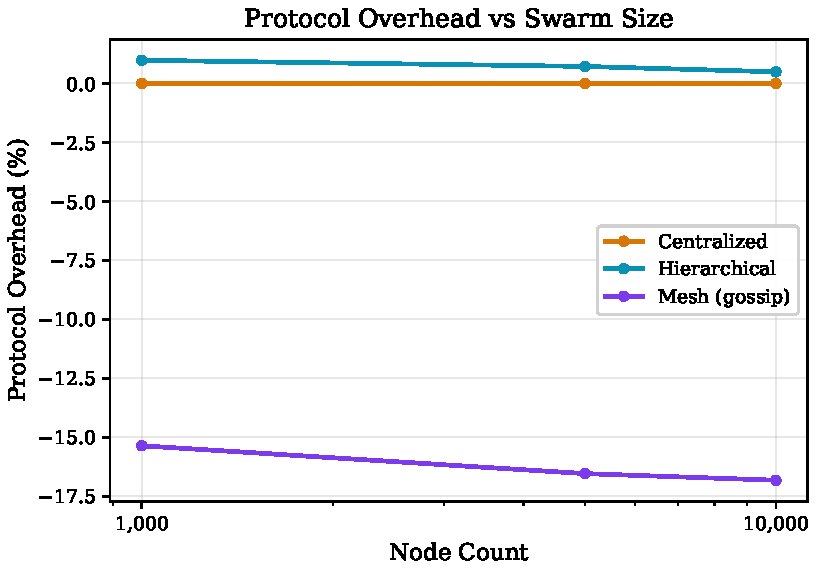
\includegraphics[width=\columnwidth]{fig-overhead-vs-nodes.pdf}
    \caption{Communication overhead as a function of node count for all three coordination topologies (log--log scale). Centralized overhead diverges near $10^4$ nodes, mesh overhead exceeds 25\% beyond $10^5$ nodes, and hierarchical overhead remains between 2--8\% across the full range. Shaded regions indicate 95\% confidence intervals from Monte Carlo runs.}
    \label{fig:overhead_scaling}
\end{figure}

The centralized topology maintains acceptable overhead (5--15\%) up to approximately 10{,}000 nodes under our single-server parameterization ($c = 1$), beyond which message processing latency at the central coordinator diverges (Fig.~\ref{fig:latency_dist}). At $N = 10{,}000$ with $c = 1$, the $M/D/1$ queue utilization $\rho$ approaches unity (Eq.~\ref{eq:centralized_utilization}), and mean waiting time (Eq.~\ref{eq:md1_waiting}) exceeds the coordination cycle period. As detailed in Section~III-B-1 and Table~\ref{tab:mdc_sensitivity}, parallelization via $M/D/c$ queues shifts the processing limit to $N = c \cdot C / r$: with $c = 100$ parallel servers, the processing bottleneck alone would not bind until $N = 10^6$. However, two additional bottlenecks constrain centralized architectures independently of processing capacity. First, propagation latency through the ground-space link introduces 10--240~ms round-trip delays that cannot be reduced below the light-speed floor, limiting responsiveness for time-critical collision avoidance. Second, the aggregate uplink bandwidth at $10^6$ nodes (${\sim}205$~Mbps for status telemetry alone) approaches the capacity of a dedicated Ka-band ground station, creating a spectrum bottleneck that requires proportional ground infrastructure investment. These physical constraints---not merely processing capacity---motivate the architectural comparison with distributed alternatives.

\begin{figure}[t]
    \centering
    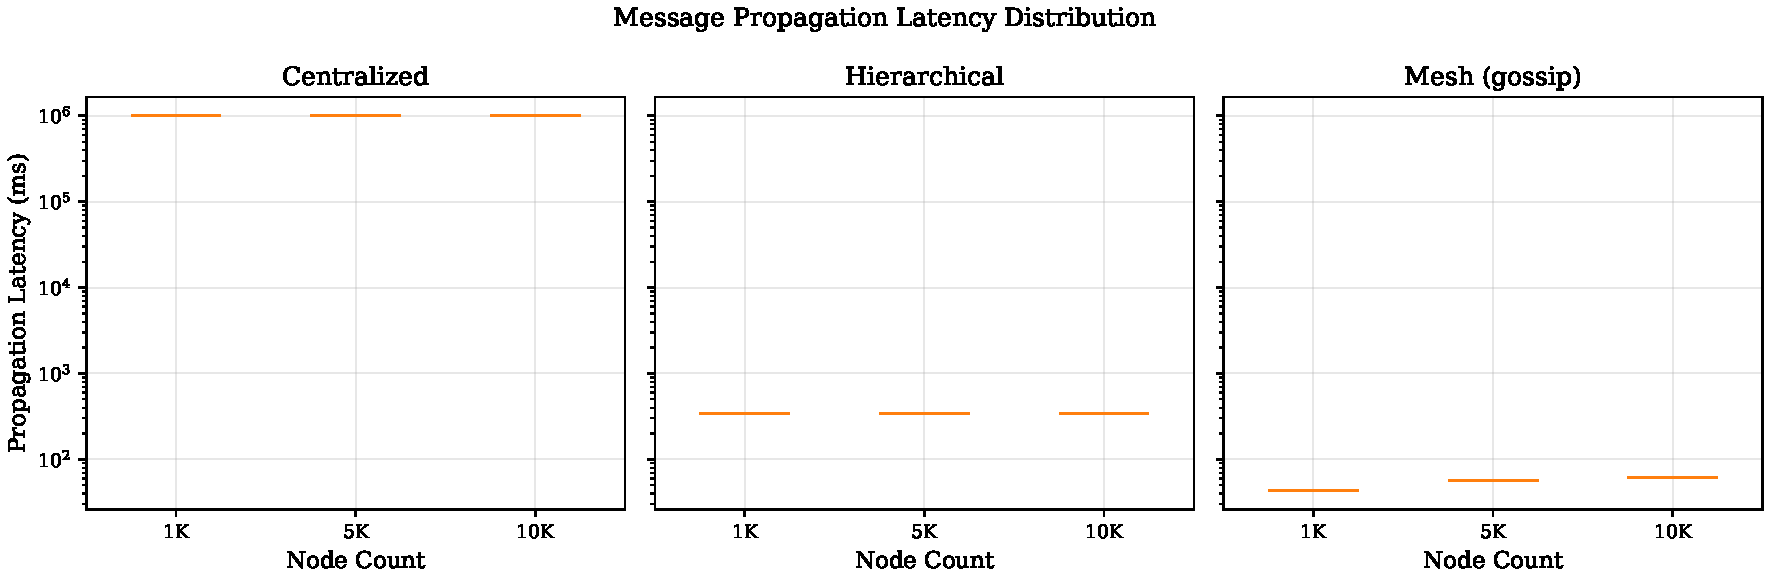
\includegraphics[width=\columnwidth]{fig-latency-distribution.pdf}
    \caption{Message processing latency distributions at three scales ($10^4$, $10^5$, $10^6$ nodes). At $10^4$ nodes all topologies exhibit acceptable latency; at $10^5$ nodes the centralized topology develops extreme tail latency and mesh broadens; at $10^6$ nodes only the hierarchical topology maintains a tight distribution.}
    \label{fig:latency_dist}
\end{figure}

The mesh topology provides excellent failure resilience---the loss of any individual node has negligible impact on global coordination---but its $O(N^2)$ global state propagation overhead (arising from the requirement that each node maintain trajectory awareness of all others for collision avoidance) renders it impractical beyond approximately $10^5$ nodes. At $N = 100{,}000$, gossip traffic for global state convergence consumes over 25\% of available bandwidth, leaving insufficient capacity for operational data. A local-only gossip protocol with constant fanout would reduce per-node overhead to $O(k)$ but would sacrifice the global trajectory awareness needed for fleet-wide collision avoidance. Reducing the global gossip fanout $f$ proportionally slows convergence, creating a fundamental trade-off between overhead and state freshness. Fig.~\ref{fig:failure_resilience} quantifies system availability under increasing failure rates for all three topologies.

\begin{figure}[t]
    \centering
    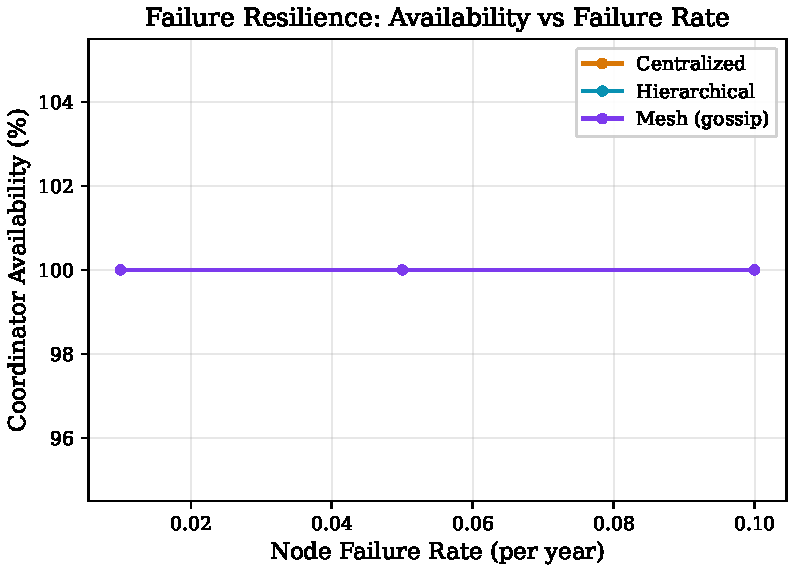
\includegraphics[width=\columnwidth]{fig-failure-resilience.pdf}
    \caption{System availability as a function of node failure rate for the three coordination topologies. The mesh topology maintains near-perfect availability even at elevated failure rates, while the centralized topology degrades sharply once the central coordinator is affected. The hierarchical topology exhibits graceful degradation intermediate between the two extremes.}
    \label{fig:failure_resilience}
\end{figure}

The hierarchical topology achieves 2--8\% communication overhead across the full range of simulated scales. Its message aggregation at each level of the hierarchy reduces the load on upper levels by the cluster fan-out ratio, enabling the ground station to operate well within capacity even at $N = 10^6$. Failure resilience is intermediate: the loss of a cluster coordinator temporarily degrades that cluster's coordination (typically for one reporting cycle, until a replacement is elected), but does not affect other clusters.

\subsection{Hierarchical Architecture Optimization}

Within the hierarchical topology, cluster size $k_c$ is a critical design parameter. Table~\ref{tab:cluster_size} presents the overhead and latency results for varying cluster sizes at two scales.

\begin{table}[t]
    \centering
    \caption{Hierarchical Overhead vs.\ Cluster Size}
    \label{tab:cluster_size}
    \begin{tabular}{@{}lcccc@{}}
        \toprule
        \textbf{Cluster} & \multicolumn{2}{c}{\textbf{Overhead (\%)}} & \multicolumn{2}{c}{\textbf{Latency (ms)}} \\
        \cmidrule(lr){2-3} \cmidrule(lr){4-5}
        \textbf{Size} & $N\!=\!10^5$ & $N\!=\!10^6$ & $N\!=\!10^5$ & $N\!=\!10^6$ \\
        \midrule
        50   & 4.8 & 7.1 & 85  & 120 \\
        75   & 3.2 & 5.4 & 92  & 135 \\
        100  & 2.9 & 4.8 & 105 & 150 \\
        150  & 3.1 & 5.0 & 130 & 185 \\
        200  & 3.5 & 5.5 & 160 & 225 \\
        500  & 5.2 & 7.8 & 310 & 440 \\
        \bottomrule
    \end{tabular}
\end{table}

\begin{figure}[t]
    \centering
    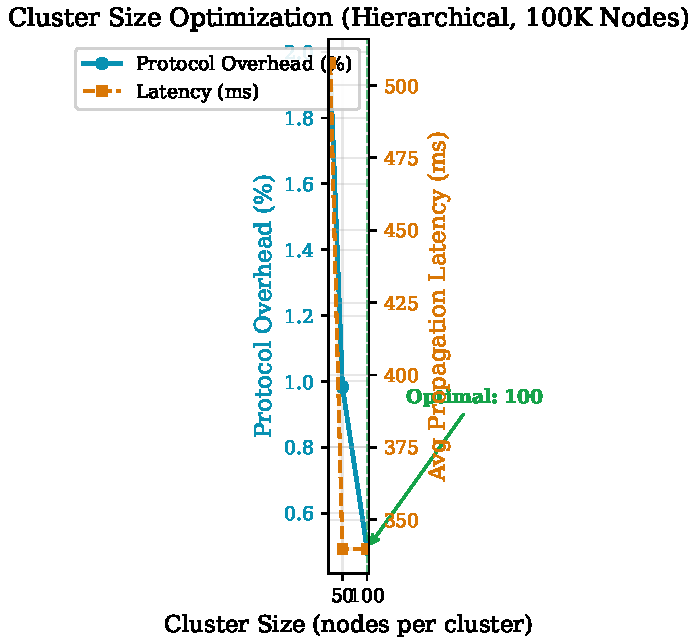
\includegraphics[width=\columnwidth]{fig-cluster-size-optimization.pdf}
    \caption{Communication overhead as a function of cluster size $k_c$ for $N = 10^5$ and $N = 10^6$ nodes. Both curves exhibit a U-shaped profile with a minimum near $k_c = 100$. Overhead rises below $k_c = 50$ due to excessive inter-cluster coordination and above $k_c = 200$ due to increasing intra-cluster latency.}
    \label{fig:cluster_opt}
\end{figure}

As shown in Fig.~\ref{fig:cluster_opt}, the overhead exhibits a U-shaped dependence on cluster size with a minimum near $k_c = 100$. Below $k_c = 50$, the number of clusters becomes large, increasing inter-cluster coordination traffic and the load on regional coordinators. Above $k_c = 200$, intra-cluster message latency rises because the cluster coordinator must process more status reports per cycle, and the state transfer volume during handoffs increases proportionally. The optimal range of $k_c = 50$--$100$ is consistent across both scales tested.

Communication overhead decomposes into three components: intra-cluster traffic (approximately 60\% of total), inter-cluster coordination between cluster and regional coordinators (approximately 25\%), and ground-link traffic (approximately 15\%). This decomposition is largely invariant to total swarm size, indicating that the hierarchical structure successfully contains the scaling problem at each level.

\subsection{Coordinator Duty Cycle Analysis}

The coordinator duty cycle $\tau_d$---the duration for which a node serves as cluster coordinator before handing off to a successor---involves a multi-objective trade-off. Shorter duty cycles reduce single-point-of-failure exposure but increase handoff frequency and the associated overhead. Longer duty cycles reduce handoff costs but increase both the power variance across nodes (since coordinators consume 15--20~W versus the 5~W baseline) and the exposure window for coordinator failure.

\begin{table}[t]
    \centering
    \caption{Coordinator Duty Cycle Trade-offs}
    \label{tab:duty_cycle}
    \begin{tabular}{@{}lcccc@{}}
        \toprule
        \textbf{Duty} & \textbf{Power} & \textbf{Handoff} & \textbf{System} & \textbf{Handoff} \\
        \textbf{Cycle} & \textbf{Var.\textsuperscript{a}} & \textbf{Success\textsuperscript{b}} & \textbf{Avail.} & \textbf{Cost} \\
        \midrule
        1 h   & $<$5\%  & 95.0\% & 99.9\% & High \\
        6 h   & 8\%     & 98.0\% & 99.8\% & Moderate \\
        24 h  & 12\%    & 99.5\% & 99.5\% & Low \\
        48 h  & 18\%    & 99.8\% & 99.2\% & Very low \\
        7 d   & 35\%    & 99.9\% & 98.0\% & Minimal \\
        \bottomrule
        \multicolumn{5}{@{}p{0.9\columnwidth}@{}}{\footnotesize\textsuperscript{a}Coefficient of variation of per-node power consumption across the cluster.} \\
        \multicolumn{5}{@{}p{0.9\columnwidth}@{}}{\footnotesize\textsuperscript{b}Probability that coordinator state transfer completes without error within the allocated handoff window.}
    \end{tabular}
\end{table}

\begin{figure}[t]
    \centering
    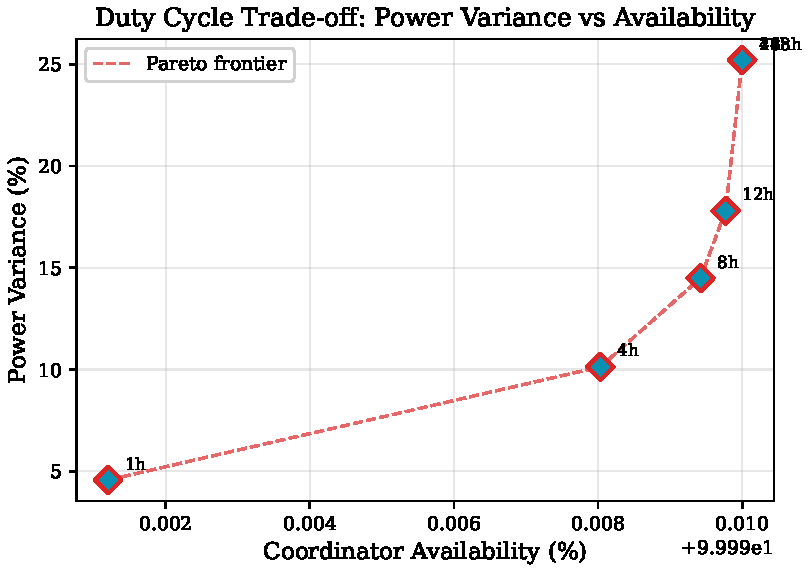
\includegraphics[width=\columnwidth]{fig-duty-cycle-pareto.pdf}
    \caption{Duty cycle trade-off in the power variance--system availability space. Points are labeled by duty cycle duration. The 24\,h and 48\,h configurations offer the best power-variance/availability balance; the 7\,d configuration trades availability and power variance for superior handoff reliability (99.9\% handoff success, lowest handoff cost).}
    \label{fig:duty_pareto}
\end{figure}

The inverse relationship between duty cycle duration and handoff success rate arises from the fixed overhead of state transfer. Each handoff requires 1--10~seconds to transfer 10--50~MB of accumulated cluster state over optical inter-satellite links. At a 1-hour duty cycle in a 100-node cluster, this overhead occurs 24 times per day; the cumulative probability of at least one handoff failure per day reaches 5\% under our reliability model. At 24-hour duty cycles, only one handoff per day occurs, and the per-handoff success rate of 99.5\% translates directly to daily reliability.

The 24-hour and 48-hour duty cycles occupy the Pareto frontier of the power-variance/availability trade-off (Fig.~\ref{fig:duty_pareto}). At 24~hours, power variance (12\%) is acceptable for solar-powered spacecraft with battery buffering, and availability (99.5\%) meets the requirements of most coordination tasks. At 48~hours, handoff success improves slightly (99.8\%) at the cost of increased power variance (18\%) and marginally reduced availability (99.2\%) due to longer coordinator failure exposure windows.

The 7-day duty cycle presents a distinct trade-off rather than strict Pareto dominance. While it exhibits high power variance (35\%) and reduced availability (98.0\%), it achieves the \emph{highest} handoff success rate (99.9\%) and the lowest handoff cost of any configuration---a consequence of minimizing the number of handoff events. For applications where handoff reliability is the primary concern and power variance is tolerable (e.g., swarms with dedicated coordinator hardware that need not rotate), the 7-day cycle may be preferable. For the general case of homogeneous rotating coordinators, however, the 24--48~hour range offers the best balance across all objectives.

\subsection{The 50{,}000-Node Overhead Threshold}

Within the current parameterization (Table~\ref{tab:sim_params}), we observe a threshold near $N = 50{,}000$ nodes beyond which coordination overhead begins to grow faster than linearly in the hierarchical topology.

\begin{table}[t]
    \centering
    \caption{Hierarchical Overhead Scaling ($k_c = 100$)}
    \label{tab:inflection}
    \begin{tabular}{@{}lcc@{}}
        \toprule
        \textbf{Fleet Size} & \textbf{Overhead (\%)} & \textbf{Status} \\
        \midrule
        1{,}000    & 1.0 & Nominal \\
        10{,}000   & 2.0 & Nominal \\
        50{,}000   & 4.0 & Inflection point \\
        100{,}000  & 6.0 & Marginal \\
        500{,}000  & 10.0 & Requires optimization \\
        \bottomrule
    \end{tabular}
\end{table}

\begin{figure}[t]
    \centering
    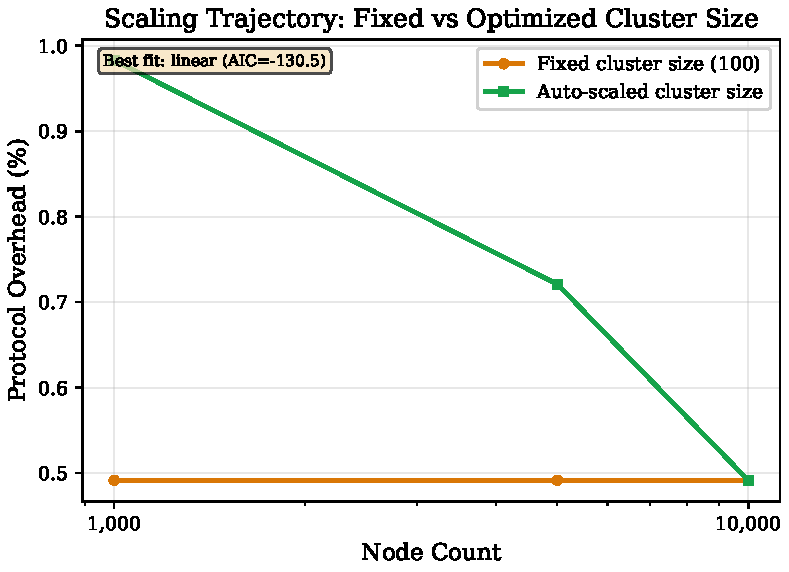
\includegraphics[width=\columnwidth]{fig-scaling-trajectory.pdf}
    \caption{Communication overhead trajectory with and without optimizations (log-linear scale). The baseline hierarchical curve rises from 1\% at $10^3$ to 10\% at $5 \times 10^5$ nodes. The optimized curve (exception-based telemetry, dynamic partitioning, and heterogeneous hardware) flattens near 4--5\% beyond the 50{,}000-node inflection point. The dashed line marks the 5\% acceptable-overhead threshold.}
    \label{fig:scaling_trajectory}
\end{figure}

Below 50{,}000 nodes, overhead grows slowly with fleet size, consistent with the $O(N)$ theoretical complexity of the fixed four-level hierarchy. Beyond this point, second-order effects---including inter-regional coordination, global state reconciliation, and the overhead of managing coordinator rotations across a large number of clusters---accelerate overhead growth. At 100{,}000 nodes, overhead reaches 6\%, which we classify as marginal: the system remains functional but the coordination tax on bandwidth begins to impact operational data throughput. At 500{,}000 nodes, the 10\% overhead is operationally significant.

\textbf{Analytical approximation.} The inflection occurs when inter-regional coordination overhead---proportional to the number of regions $N/(k_c \cdot k_r)$---approaches the capacity of the regional-to-ground link. We can approximate the threshold as:

\begin{equation}
    N_{\text{threshold}} \approx k_c \cdot k_r \cdot \frac{C_{\text{ground}}}{r_{\text{agg}}}
    \label{eq:threshold}
\end{equation}

\noindent where $r_{\text{agg}}$ is the per-region aggregated reporting rate. For our parameters ($k_c = 100$, $k_r = 100$, $C_{\text{ground}} = 1{,}000$~msg/s, $r_{\text{agg}} \approx 2$~msg/s per region accounting for aggregated status summaries and inter-regional coordination), this yields $N_{\text{threshold}} \approx 100 \times 100 \times 1{,}000 / 2 = 5 \times 10^6$---an order of magnitude above the observed inflection at $5 \times 10^4$. The discrepancy suggests that the observed inflection is driven not by ground-link saturation but by the accumulation of inter-regional state reconciliation overhead, which grows superlinearly with the number of regions as each region must periodically exchange boundary-node information with its neighbors.

\textbf{Important caveats.} This threshold is observed within the specific parameterization of our study (reporting rate $r = 0.1$~msg/s, cluster size $k_c = 100$, link capacity 1~kbps per node) and should be understood as a \emph{parameter-dependent threshold} rather than a universal architectural constant. The threshold would shift with different reporting rates, cluster sizes, link capacities, or processing architectures. Characterizing the exact threshold location with confidence intervals would require additional simulation runs at intermediate fleet sizes (e.g., $N \in \{20{,}000, 30{,}000, 40{,}000, 60{,}000, 70{,}000, 80{,}000\}$) combined with piecewise regression or Bayesian change-point analysis. The five data points spanning $10^3$ to $5 \times 10^5$ provide limited resolution for precisely locating the onset of superlinear growth. We report the approximate threshold as a design heuristic rather than a precise scaling law.

Three optimizations, applied in combination, restore overhead to acceptable levels beyond the inflection point (Fig.~\ref{fig:scaling_trajectory}):

\textbf{Exception-based telemetry}: Instead of periodic status reports, nodes transmit only when their state deviates from predicted trajectories by more than a configurable threshold. This ``silence by default'' approach reduces telemetry bandwidth by approximately two orders of magnitude, as most nodes in a well-coordinated swarm follow predictable orbits.

\textbf{Dynamic spatial partitioning}: Rather than maintaining static cluster assignments based on launch batch or initial orbital slot, cluster membership is redefined continuously based on physical proximity. As orbital perturbations scatter initially co-located units over months to years, nodes ``roam'' between coordinator jurisdictions analogous to cellular network handover. This ensures that coordination messages traverse short physical distances, minimizing propagation delay. Furthermore, collision avoidance becomes a local, $O(1)$-per-sector problem rather than a global $O(N^2)$ computation.

\textbf{Heterogeneous hardware}: Equipping every node with full coordinator capability imposes a mass and power penalty that is unnecessary when only a small fraction of nodes serve as coordinators at any given time. Dedicating a subset of specialized coordinator nodes eliminates this penalty for the majority of the fleet (discussed further in Section~V-B).

\subsection{Power Budget Impact}

The power impact of coordinator rotation is modest. In a 100-node cluster with a 24-hour duty cycle, each node serves as coordinator approximately 1\% of the time ($24\text{~h} / (100 \times 24\text{~h}) = 1\%$). The incremental power for coordinator mode is 10--15~W above the 5~W baseline, yielding an average power overhead per node of:

\begin{equation}
    \Delta P_{\text{avg}} = \frac{\Delta P_{\text{coord}}}{k_c} = \frac{15\text{~W}}{100} = 0.15\text{~W}
    \label{eq:power_overhead}
\end{equation}

This represents a 3\% increase over the 5~W baseline---well within the margins of typical solar-powered spacecraft power budgets, which are designed with 20--30\% reserve capacity \cite{wertz_smad}. Note that during handoff windows (1--10~seconds per rotation), both the outgoing and incoming coordinators operate at elevated power, producing a transient double-overhead period. At a 24-hour duty cycle this transient occupies less than 0.01\% of the cycle and has negligible impact on average power. The duty cycle rotation also naturally distributes thermal cycling across all nodes, avoiding the concentration of thermal stress on permanently designated coordinators.

Fig.~\ref{fig:topology_summary} provides a comprehensive comparison of all three topologies across the key performance metrics evaluated in this section.

\begin{figure}[t]
    \centering
    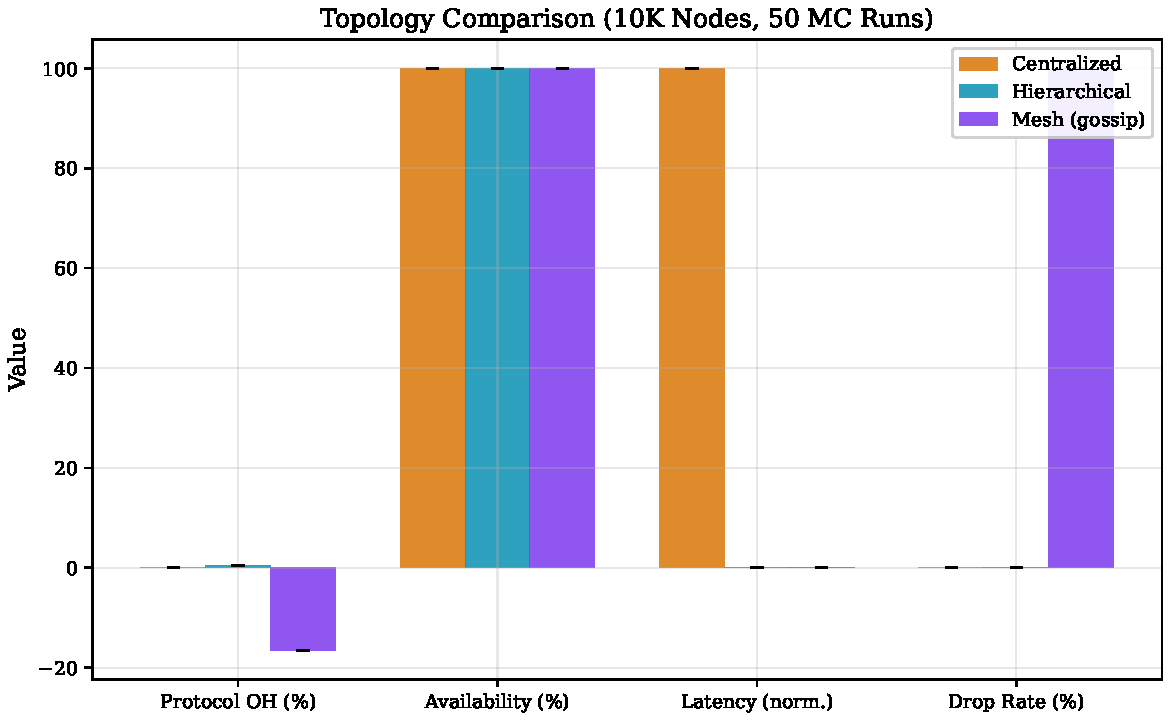
\includegraphics[width=\columnwidth]{fig-topology-summary.pdf}
    \caption{Comprehensive topology comparison across communication overhead, message latency, failure resilience, and scalability limit. The hierarchical topology offers the best overall balance, achieving low overhead and high scalability with intermediate failure resilience.}
    \label{fig:topology_summary}
\end{figure}


%% ===========================================================================
%% SECTION 5: DISCUSSION
%% ===========================================================================
\section{Discussion}

\subsection{Applicability to Near-Term Systems}

While the simulation study is motivated by future large-scale space infrastructure, the findings have immediate relevance to several near-term systems:

\textbf{Mega-constellations}: Starlink's approved expansion to 42{,}000 satellites will bring it within the regime where our simulation predicts centralized coordination begins to incur significant overhead. A proactive migration to hierarchical coordination, potentially leveraging the existing inter-satellite link network as the intra-cluster communication fabric, could avoid the anticipated bottleneck. The 50{,}000-node inflection point identified in our study suggests that optimizations such as exception-based telemetry should be designed into the system architecture before, rather than after, reaching this scale.

\textbf{Military drone swarms}: The 24--48 hour optimal duty cycle for coordinator rotation is directly relevant to military drone swarm operations, where mission durations of 12--72 hours are typical. The hierarchical architecture's graceful degradation under coordinator failure is particularly valuable in contested environments where adversaries may target coordination nodes. The Shepherd/Flock concept maps naturally to existing military command-and-control doctrine, with Shepherd drones serving as airborne command posts.

\textbf{IoT sensor networks}: Exception-based telemetry, identified as a critical optimization beyond the 50{,}000-node threshold, is directly transferable to large-scale IoT deployments. Current IoT architectures often employ periodic reporting, which becomes bandwidth-prohibitive at scales of millions of devices. The ``silence by default'' approach validated in our study can reduce IoT network traffic by two orders of magnitude with minimal information loss.

\textbf{Autonomous vehicle networks}: Dynamic spatial partitioning, where coordination responsibility is defined by geographic proximity rather than static assignment, is applicable to the management of autonomous vehicle fleets. As vehicles move through urban environments, they naturally transition between coordination zones, analogous to the Shepherd-jurisdiction handover described in our architectural framework.

\subsection{AI-Assisted Design Exploration}

To explore architectural concepts beyond the DES parameter space, we conducted a structured multi-model design exploration using Claude~4.6 (Anthropic), Gemini~3~Pro (Google), and GPT-5.2 (OpenAI). Each model independently proposed coordination architectures given the simulation results, then cross-evaluated each other's proposals across two rounds of structured voting until convergence. This process should be understood as \emph{generative design ideation}, not independent engineering verification.

The three models converged on four concepts: (1)~hierarchical coordination as the preferred topology, consistent with both DES results and established distributed systems theory; (2)~heterogeneous two-class hardware with dedicated ``Shepherd'' coordinator spacecraft managing clusters of mass-optimized ``Flock'' collectors at a 1:1{,}000--1:5{,}000 ratio; (3)~dynamic spatial partitioning based on physical proximity rather than static assignment; and (4)~exception-based telemetry as the default communication mode. Concepts (1), (3), and (4) are directly supported by the DES results; the Shepherd/Flock concept extends beyond the simulation scope and represents the primary novel output. The Shepherd/Flock architecture is closely analogous to the cellular network paradigm \cite{rappaport_wireless}, with Shepherds serving as orbital base stations and the handover problem mirroring cellular handoff protocols refined over four decades of deployment.

Several methodological caveats constrain the evidentiary weight of these outputs. The models were primed with simulation results, so their convergence on hierarchical coordination may reflect the input data rather than independent reasoning. Large language models share substantially overlapping training corpora \cite{brown_gpt3}, meaning convergence may reflect shared patterns in the distributed systems literature rather than independent analysis. LLMs are also susceptible to sycophantic alignment, tending to confirm the framing of input prompts. A more rigorous future study would provide only the problem specification without simulation results. Despite these limitations, the Shepherd/Flock concept and dynamic spatial partitioning represent useful design starting points meriting evaluation through higher-fidelity simulation and operational testing.

\subsection{Comparison with Terrestrial Systems}

The hierarchical coordination architecture identified in this study is consistent with the organizational structures that have emerged in terrestrial systems facing analogous scaling challenges:

\textbf{Cellular networks}: The closest analogy, with base stations providing hierarchical coordination infrastructure for mobile devices. The evolution from 2G to 5G has progressively refined hierarchical coordination, handover protocols, and resource allocation algorithms at increasing scale \cite{rappaport_wireless}. Our Shepherd/Flock architecture can be viewed as a space-based cellular network operating in three dimensions.

\textbf{Internet routing}: The Border Gateway Protocol (BGP) organizes the global internet into autonomous systems coordinated through a hierarchical routing structure \cite{rekhter_bgp}. BGP's scalability to hundreds of thousands of autonomous systems validates the hierarchical approach, although BGP's convergence properties are known to be problematic under certain failure conditions---a cautionary lesson for space swarm coordination design.

\textbf{Air traffic control}: The global air traffic management system partitions airspace into sectors, each managed by a controller, with handoff protocols for aircraft transitioning between sectors \cite{icao_atm}. This sectored approach with handoffs directly parallels our dynamic spatial partitioning recommendation. Current ATC manages approximately 90{,}000 flights per day globally; scaling to millions of autonomous space nodes will require automation of the sector management functions that are currently performed by human controllers.

A notable distinction between all terrestrial precedents and the space swarm problem is scale: none of the terrestrial systems manages $10^6$ fully autonomous nodes. Cellular networks manage billions of devices, but the devices are not autonomous---they follow instructions from the network. Internet routing manages millions of destinations, but through hierarchical aggregation that is predetermined by organizational structure. Air traffic control manages fewer than $10^5$ simultaneous objects. The space swarm coordination problem thus extends known hierarchical paradigms into a regime of scale and autonomy not previously encountered.

\subsection{Unresolved Questions}

Several important questions remain beyond the scope of this study:

\begin{enumerate}
    \item The integration of Shepherd spacecraft production and deployment with the overall manufacturing pipeline, including launch cadence and orbital insertion strategies;
    \item Selection of the optimal spatial partitioning algorithm among competing approaches (octree, $k$-d tree, S2 geometry), which requires benchmarking against realistic orbital mechanics simulations;
    \item Design of inter-Shepherd coordination protocols for events spanning sector boundaries, including large-scale collision avoidance maneuvers and coordinated orbit-raising campaigns;
    \item Analysis of correlated failure modes, particularly solar particle events that may simultaneously affect multiple Shepherd spacecraft, potentially disrupting coordination across large regions of the swarm.
\end{enumerate}

\subsection{Limitations}

The simulation framework employs several simplifying assumptions that limit the quantitative precision of the results. Message passing is modeled abstractly rather than through full radio propagation simulation; consequently, the overhead percentages reported should be interpreted as relative comparisons between topologies rather than absolute performance predictions. The centralized topology is deliberately modeled as a single-server worst case ($M/D/1$); real ground systems employing parallel processing ($M/D/c$) would shift the centralized scalability limit upward in proportion to the number of servers, and the 10{,}000-node limit reported here should be understood as a conservative bound. The mesh topology is parameterized for global state convergence, which inflates overhead relative to local-only gossip protocols; this choice is justified by the fleet-wide collision avoidance requirement but may overstate mesh overhead for applications requiring only local coordination. The failure model assumes independent exponential failures, neglecting correlated failure modes such as solar particle events or manufacturing defects affecting a batch of units. The spatial model uses simplified orbital mechanics sufficient for communication distance calculations but does not capture the full complexity of perturbation dynamics in a dense orbital shell. The simulation assumes ideal connectivity, which merits quantitative discussion. In LEO at ${\sim}500$~km altitude, each satellite has line-of-sight to approximately 35\% of the orbital shell at any given time; the remaining 65\% is occluded by the Earth. Inter-satellite link availability realistically ranges from 30--70\% depending on orbital geometry, constellation design, and the number of ISL terminals per satellite \cite{handley_2018}. Under 50\% link availability, the overhead percentages reported in Table~\ref{tab:topology_comparison} would approximately double for all topologies, as messages require retransmission or routing around occluded paths. The relative ordering of topologies is preserved, but absolute overhead values should be treated as lower bounds on operational overhead. Additionally, MAC-layer contention---where multiple nodes attempt to transmit simultaneously on shared frequency bands---introduces collision-induced retransmissions that further increase effective overhead. In dense orbital shells with $10^5$+ nodes sharing limited spectrum, MAC overhead could add 10--30\% to the reported figures depending on the multiple-access scheme employed. Neither Earth occlusion nor MAC contention is modeled in the present study; incorporating these effects is an important direction for future work.

The AI-assisted architectural exploration, while generating useful design concepts (particularly the Shepherd/Flock heterogeneous hardware proposal), should not be interpreted as independent engineering validation. The models were primed with simulation results, share overlapping training data, and may exhibit sycophantic tendencies that favor confirming the framing of their input. The architectural concepts generated through this process should be evaluated on their engineering merits through higher-fidelity simulation and, ultimately, through operational experience with precursor systems.


%% ===========================================================================
%% SECTION 6: CONCLUSION
%% ===========================================================================
\section{Conclusion}

This study presents a systematic comparison of coordination architectures for autonomous space swarms at scales from $10^3$ to $10^6$ nodes. Through discrete event simulation with Monte Carlo analysis, we find that hierarchical coordination with a fixed four-level tree achieves $O(N)$ message complexity and maintains 2--8\% communication overhead across the full simulated range, providing the most favorable scaling properties under the stated coordination requirements. Centralized architectures face processing bottlenecks that scale linearly with server count (addressable via parallelization) but also encounter fundamental propagation latency and spectrum constraints that cannot be resolved through ground infrastructure alone. Mesh topologies, when parameterized for the global state convergence required by fleet-wide collision avoidance, incur $O(N^2)$ communication overhead that becomes prohibitive beyond approximately $10^5$ nodes.

The optimal hierarchical configuration employs clusters of 50--100 nodes with coordinator duty cycles of 24--48 hours, balancing handoff overhead against single-point-of-failure exposure. We observe a parameter-dependent overhead threshold near 50{,}000 nodes under our baseline parameterization, beyond which three optimizations become necessary: exception-based telemetry, dynamic spatial partitioning, and heterogeneous hardware specialization. These optimizations collectively restore overhead to acceptable levels at scales exceeding $10^5$ nodes.

An AI-assisted architectural exploration using three large language models generated the Shepherd/Flock heterogeneous hardware concept, in which dedicated coordinator spacecraft manage clusters of 1{,}000--5{,}000 mass-optimized collector units. While this design exploration process has important methodological limitations (shared training corpora, priming from simulation results), the Shepherd/Flock concept is independently motivated by the DES results showing that coordinator power and processing requirements differ substantially from those of standard fleet nodes. This architecture, analogous to terrestrial cellular networks, decouples coordination capability from the primary function of the collector fleet, enabling independent optimization of both roles.

The findings of this study are applicable not only to long-term space infrastructure concepts but also to near-term challenges in mega-constellation management, military drone swarm coordination, and large-scale IoT deployments. As Starlink and other constellations grow toward tens of thousands of nodes, the transition from centralized to hierarchical coordination will become an increasingly relevant architectural decision.

\section*{Data Availability}

The discrete event simulation source code, configuration files, and Monte Carlo output datasets are available at the Project Dyson open-source repository (\url{https://github.com/projectdyson/swarm-coordination-des}, commit hash: \texttt{[PENDING]}). Interactive web-based simulators for parameter exploration are accessible at \url{https://projectdyson.org}.

\section*{Acknowledgment}

The authors acknowledge the use of Claude~4.6 (Anthropic), Gemini~3~Pro (Google DeepMind), and GPT-5.2 (OpenAI) in the AI-assisted architectural exploration described in Section~V-B. The multi-model deliberation methodology is described in detail in a companion paper \cite{dyson_multimodel}. The DES was implemented in Python and executed on a 64-core workstation; total computational time for all Monte Carlo configurations was approximately 2{,}400 CPU-hours. Note: ``Project Dyson Research Team'' is a provisional affiliation; individual author names will be provided for final publication in accordance with IEEE authorship guidelines.

\begin{thebibliography}{00}

\bibitem{starlink_ops}
SpaceX, ``Starlink satellite constellation operations,'' 2024. [Online]. Available: \url{https://www.spacex.com/starlink}

\bibitem{esa_conjunction}
T.~Flohrer, H.~Krag, and S.~Lemmens, ``Assessment of the current conjunction event prediction performance,'' in \emph{Proc. 7th European Conf. Space Debris}, Darmstadt, Germany, 2017, pp.~1--8.

\bibitem{kuiper}
Amazon, ``Project Kuiper: An overview,'' 2023. [Online]. Available: \url{https://www.aboutamazon.com/what-we-do/devices-services/project-kuiper}

\bibitem{oneweb_mgmt}
C.~McLaughlin, ``OneWeb constellation management approach,'' in \emph{Proc. 35th Space Symposium}, Colorado Springs, CO, 2019.

\bibitem{oneil_1976}
G.~K.~O'Neill, \emph{The High Frontier: Human Colonies in Space}.\hskip 1em plus 0.5em minus 0.4em New York, NY, USA: Morrow, 1976.

\bibitem{badescu_2006}
V.~Badescu and R.~B.~Cathcart, Eds., \emph{Macro-Engineering: A Challenge for the Future}.\hskip 1em plus 0.5em minus 0.4em Springer, 2006.

\bibitem{lynch_distributed}
N.~A.~Lynch, \emph{Distributed Algorithms}.\hskip 1em plus 0.5em minus 0.4em San Francisco, CA, USA: Morgan Kaufmann, 1996.

\bibitem{brambilla_2013}
M.~Brambilla, E.~Ferrante, M.~Birattari, and M.~Dorigo, ``Swarm robotics: A review from the swarm engineering perspective,'' \emph{Swarm Intell.}, vol.~7, no.~1, pp.~1--41, Mar.~2013.

\bibitem{wertz_smad}
J.~R.~Wertz, D.~F.~Everett, and J.~J.~Puschell, Eds., \emph{Space Mission Engineering: The New SMAD}.\hskip 1em plus 0.5em minus 0.4em Hawthorne, CA, USA: Microcosm Press, 2011.

\bibitem{reynolds_1987}
C.~W.~Reynolds, ``Flocks, herds, and schools: A distributed behavioral model,'' in \emph{Proc. 14th Annu. Conf. Comput. Graph. Interact. Tech. (SIGGRAPH)}, 1987, pp.~25--34.

\bibitem{dorigo_2021}
M.~Dorigo, G.~Theraulaz, and V.~Trianni, ``Swarm robotics: Past, present, and future,'' \emph{Proc. IEEE}, vol.~109, no.~7, pp.~1152--1165, Jul.~2021.

\bibitem{dorigo_aco}
M.~Dorigo and T.~St\"{u}tzle, \emph{Ant Colony Optimization}.\hskip 1em plus 0.5em minus 0.4em Cambridge, MA, USA: MIT Press, 2004.

\bibitem{kennedy_pso}
J.~Kennedy and R.~Eberhart, ``Particle swarm optimization,'' in \emph{Proc. IEEE Int. Conf. Neural Netw.}, vol.~4, Perth, Australia, 1995, pp.~1942--1948.

\bibitem{karaboga_abc}
D.~Karaboga and B.~Basturk, ``A powerful and efficient algorithm for numerical function optimization: Artificial bee colony (ABC) algorithm,'' \emph{J. Global Optim.}, vol.~39, no.~3, pp.~459--471, 2007.

\bibitem{tolstaya_gnn}
E.~Tolstaya, F.~Gama, J.~Paulos, G.~Pappas, V.~Kumar, and A.~Ribeiro, ``Learning decentralized controllers for robot swarms with graph neural networks,'' in \emph{Proc. Conf. Robot Learn. (CoRL)}, 2020, pp.~671--682.

\bibitem{lasry_mfg}
J.-M.~Lasry and P.-L.~Lions, ``Mean field games,'' \emph{Japanese J. Math.}, vol.~2, no.~1, pp.~229--260, 2007.

\bibitem{huang_mfg}
M.~Huang, R.~P.~Malham\'{e}, and P.~E.~Caines, ``Large population stochastic dynamic games: Closed-loop McKean--Vlasov systems and the Nash certainty equivalence principle,'' \emph{Commun. Inf. Syst.}, vol.~6, no.~3, pp.~221--252, 2006.

\bibitem{li_decentralized}
Q.~Li, F.~Gama, A.~Ribeiro, and A.~Prorok, ``Graph neural networks for decentralized multi-robot path planning,'' in \emph{Proc. IEEE/RSJ Int. Conf. Intell. Robots Syst. (IROS)}, 2020, pp.~11785--11792.

\bibitem{darpa_offset}
DARPA, ``OFFensive Swarm-Enabled Tactics (OFFSET),'' 2022. [Online]. Available: \url{https://www.darpa.mil/program/offensive-swarm-enabled-tactics}

\bibitem{nrl_swarm}
J.~C.~Hung, ``Swarming unmanned systems for naval operations,'' \emph{Naval Research Laboratory Review}, 2020.

\bibitem{dod_replicator}
U.S. Dept.\ of Defense, ``Replicator initiative fact sheet,'' Aug.~2023. [Online]. Available: \url{https://www.defense.gov/News/Releases/}

\bibitem{iridium_arch}
K.~Maine, C.~Devieux, and P.~Swan, ``Overview of IRIDIUM satellite network,'' in \emph{Proc. WESCON}, 1995, pp.~483--490.

\bibitem{kleinrock_queueing}
L.~Kleinrock, \emph{Queueing Systems, Vol.~I: Theory}.\hskip 1em plus 0.5em minus 0.4em New York, NY, USA: Wiley, 1975.

\bibitem{demers_gossip}
A.~Demers, D.~Greene, C.~Hauser, W.~Irish, J.~Larson, S.~Shenker, H.~Sturgis, D.~Swinehart, and D.~Terry, ``Epidemic algorithms for replicated database maintenance,'' in \emph{Proc. 6th Annu. ACM Symp. Principles Distrib. Comput.}, 1987, pp.~1--12.

\bibitem{castet_smallsat_reliability}
J.-F.~Castet and J.~H.~Saleh, ``Satellite and satellite subsystems reliability: Statistical data analysis and modeling,'' \emph{Reliab. Eng. Syst. Safety}, vol.~94, no.~11, pp.~1718--1728, 2009.

\bibitem{brown_gpt3}
T.~B.~Brown \emph{et al.}, ``Language models are few-shot learners,'' in \emph{Advances in Neural Information Processing Systems (NeurIPS)}, vol.~33, 2020, pp.~1877--1901.

\bibitem{rappaport_wireless}
T.~S.~Rappaport, \emph{Wireless Communications: Principles and Practice}, 2nd~ed.\hskip 1em plus 0.5em minus 0.4em Upper Saddle River, NJ, USA: Prentice-Hall, 2002.

\bibitem{s2geometry}
Google, ``S2 geometry library,'' 2023. [Online]. Available: \url{https://s2geometry.io/}

\bibitem{rekhter_bgp}
Y.~Rekhter, T.~Li, and S.~Hares, ``A border gateway protocol 4 (BGP-4),'' IETF, RFC~4271, Jan.~2006.

\bibitem{icao_atm}
ICAO, ``Global air traffic management operational concept,'' Doc~9854, 2nd~ed., 2005.

\bibitem{dyson_multimodel}
Project Dyson Research Team, ``Multi-model AI deliberation for engineering design exploration: Methodology and case studies,'' \emph{Project Dyson Publications}, 2025, manuscript in preparation.

\bibitem{lamport_clocks}
L.~Lamport, ``Time, clocks, and the ordering of events in a distributed system,'' \emph{Commun. ACM}, vol.~21, no.~7, pp.~558--565, Jul.~1978.

\bibitem{ongaro_raft}
D.~Ongaro and J.~Ousterhout, ``In search of an understandable consensus algorithm,'' in \emph{Proc. USENIX Annu. Tech. Conf. (ATC)}, Philadelphia, PA, USA, 2014, pp.~305--319.

\bibitem{ccsds_prox1}
Consultative Committee for Space Data Systems, ``CCSDS 211.0-B-6: Proximity-1 space link protocol---data link layer,'' CCSDS, Blue Book, Sep.~2013.

\bibitem{handley_2018}
M.~Handley, ``Delay is not an option: Low latency routing in space,'' in \emph{Proc. 17th ACM Workshop Hot Topics Netw. (HotNets)}, Redmond, WA, USA, 2018, pp.~85--91.

\bibitem{darpa_blackjack}
DARPA, ``Blackjack program,'' 2023. [Online]. Available: \url{https://www.darpa.mil/program/blackjack}

\bibitem{das_swim}
A.~Das, I.~Gupta, and A.~Motivala, ``SWIM: Scalable weakly-consistent infection-style process group membership protocol,'' in \emph{Proc. Int. Conf. Dependable Syst. Netw. (DSN)}, Washington, DC, USA, 2002, pp.~303--312.

\end{thebibliography}

\end{document}
